\section{Измерение формфактора полулептонных распадов $\Lambda_c$}

Процедура измерения формфакторов в распадах $\Lambda_c \to \Lambda l \nu_l$
уловому распредлению. Переменные углового распределения представлены 
на (рис. \ref{lc_l_l_nu:def}). 

\begin{figure}[H]
    \centering
    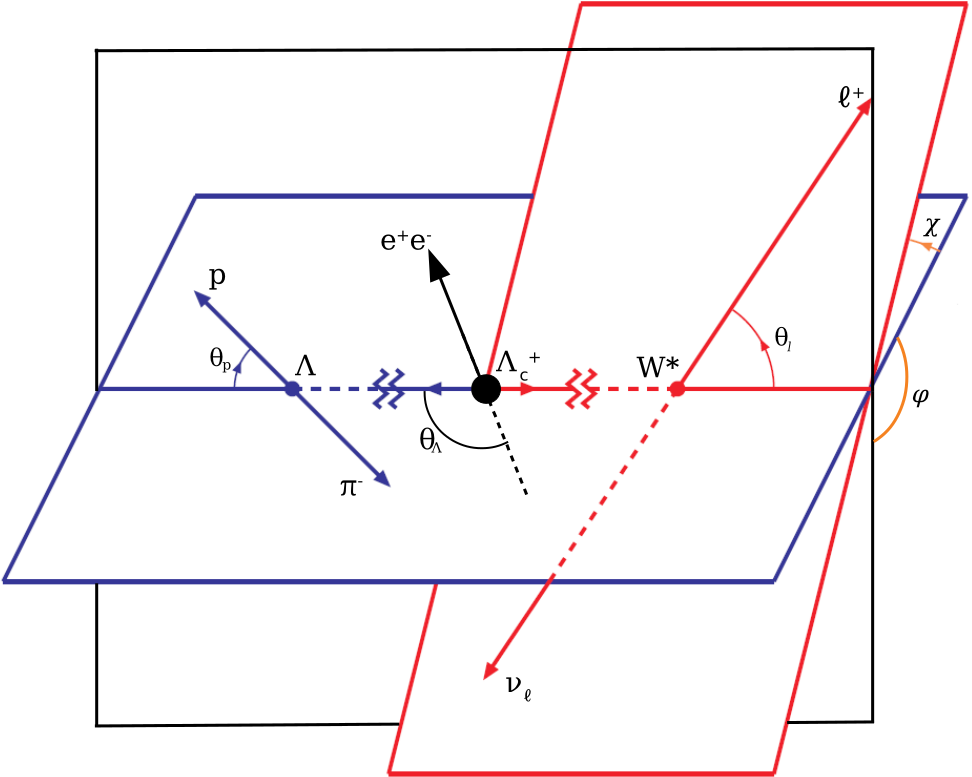
\includegraphics[width=0.7\linewidth]{img/lc_l_l_nu_def.png}
    \caption{Определение переменных углового распределения в распадах  $\Lambda_c \to \Lambda l \nu_l$.}
    \label{lc_l_l_nu:def}
\end{figure}

Амплитуда распадов 
$\Lambda_c \to \Lambda W^*, W^* \to l^+ \nu_l, \Lambda \to p \pi$:


\begin{equation}
    M_{\lambda_{\Lambda_c}\lambda_{p}\lambda_{l}\lambda_{\nu}} 
    = 
    \sum_{\lambda_{\Lambda},J,\lambda_{W}} H_{\lambda_{\Lambda},\lambda_{W}} D^{\frac{1}{2} \dagger}_{\lambda_{\Lambda_c},\lambda_{\Lambda}-\lambda_{W}}(\phi_{\Lambda}, \theta_{\Lambda}, -\phi_{\Lambda}) B_{\lambda_{p}} D^{\frac{1}{2} \dagger}_{\lambda_{\Lambda},\lambda_{p}}(\phi_{p}, \theta_{p}, -\phi_{p}) h_{\lambda_{l},\lambda_{\nu}} D^{J \dagger}_{\lambda_{W},\lambda_{l}-\lambda_{\nu}}(\phi_{l}, \theta_{l}, -\phi_{l}),
\end{equation}


где $\theta_l, \phi_l$ --- полярный и азимутальный углы импульса лептона 
в системе отсчёта  $W^*$-бозона, имеющую ось $z$, которая направлена 
противоположно импульсу $\Lambda^+_c $-бариона, 
$\lambda_l$ --- спиральность лептона, 
$\lambda_\nu$ --- спиральность нейтрино, 
которая принимает значения $-\frac{1}{2}$ у $\nu_l$, $\frac{1}{2}$ у $\bar \nu_l$, 
то есть зависит от знака заряда. 
Для вычисления спиральной амплитуды $h_{\lambda_l, \lambda_\nu}$, 
в системе покоя $W^*$-бозона, ось $z$ направлена вдоль импульса лептона 
$\vec{p}_l$ и использовались выражения биспиноров:

\begin{equation}
    \bar{u}_l\inner{\pm \frac{1}{2}} = \sqrt{E_l + m_l} \inner{\chi^{\dagger}_{\pm}, \frac{\mp |\vec{p}_l|}{E_l + m_l} \chi^{\dagger}_{\pm}}, 
    \quad 
    \bar{u}_l\inner{-\frac{1}{2}} = \sqrt{E_\nu} \inner{\chi^{\dagger}_{-}, \chi^{\dagger}_{-}},
\end{equation}
\begin{equation}
    v_l\inner{\pm \frac{1}{2}} = \sqrt{E_l + m_l} \inner{ \frac{\mp \abs{\vec{p}_l}}{E_l + m_l} \chi_{\pm}, \chi_{\pm} },
    \quad
    v_\nu\inner{+\frac{1}{2}} = \sqrt{E_\nu} \inner{-\chi_-, -\chi_-},
\end{equation}
\begin{equation}
    v_\nu\inner{+\frac{1}{2}} = \sqrt{E_\nu} \inner{-\chi_-, -\chi_-},
\end{equation}

4-векторы поляризации виртуального $W$-бозона: $\epsilon^\mu(t) = (1; 0, 0, 0), \epsilon^\mu(0) = (0; 0, 0, 1), \epsilon^\mu(\pm 1) = \frac{1}{\sqrt{2}} (0; \mp 1, -i, 0)$. 
Вследствие сохранения полного момента импульса $\lambda_W = \lambda_l - \lambda_\nu$ и вида слабого тока из СМ:

\begin{equation}
    h_{\lambda_l = \frac{1}{2}, \lambda_\nu = \frac{1}{2}} = \bar{u}_l\inner{-\frac{1}{2}} \gamma^\mu (1 + \gamma_5) v_\nu \inner{+\frac{1}{2}}
    \begin{cases}
    \epsilon_\mu(-1) \\
    \epsilon_\mu(t), \epsilon_\mu(0)
    \end{cases},
\end{equation}
\begin{equation}
    h_{\lambda_l = \pm \frac{1}{2}, \lambda_\nu = - \frac{1}{2}} = \bar{u}_l \inner{- \frac{1}{2}} \gamma^\mu (1 + \gamma_5) v_l \inner{\pm \frac{1}{2}}
    \begin{cases}
    \epsilon_\mu(1) \\
    \epsilon_\mu(t), \epsilon_\mu(0)
    \end{cases}.
\end{equation}

cпиральные амплитуды $h_{\lambda_l,\lambda_\nu}$ подразделяются на два случая, связанные
с произошедшим или не произошедшим переворотом спина лептона, то
есть изменением его спиральности на противоположную после распада $W^*$-бозона:

\begin{eqnarray}
    \text{без переворота спина} \inner{\lambda_W = \mp 1}: \ \abs{h_{\lambda_l = \mp 1/2, \lambda_\nu = \pm 1/2}}^2 = 8 \inner{q^2 - m_l^2}\\
    \text{без переворота спина} \inner{\lambda_W = t, 0}: \ \abs{h_{\lambda_l = \pm 1/2, \lambda_\nu = \pm 1/2}}^2 = 8 \cfrac{m_l^2}{2q^2}\inner{q^2 - m_l^2}
\end{eqnarray}

Так как порядка сотни восстановленных сигнальных событий 
недостаточно для измерения всех шести формфакторов в общем случае, 
были сделаны предположения:

\newdot $m_l = 0$;

\newdot $H_{\lambda_\Lambda \lambda_W} \in \re$;

\newdot Распад $\Lambda_c \to \Lambda l \nu_l$ происходит согласно теории тяжелых квакров тоесть $c \to s W^*$;

\newdot Вид формфакторов соответствует модели $KK$ согласованой с торией тяжелых кварков.

Предоложения, писанные выше были также сделаны в работе \cite{CLEO2023}, но в отличие от них 
в данной работе не делается предположения о равномерном распределении направления спина $\Lambda$,
а распределен согласно измерениям продленным в разделе \ref{helisity:Lambda}.

Проделывая вычиления аналогичные \ref{helisity:amplitud:Lam}-\ref{spin:Lam:pdf} получим из:

\begin{eqnarray}
    \frac{d\Gamma}{dq^2 d\cos\theta_\ell d\cos\theta_p d\cos\theta_d d\phi_\ell d\phi_p d\chi} = 
    p\sum_{\lambda_W \lambda_l \lambda_\nu } \abs{M_{\lambda_{\Lambda_c}\lambda_{p}\lambda_{l}\lambda_{\nu}} }^2
\end{eqnarray}

\begin{eqnarray}
    d\Gamma = \cfrac{1+P_L}{2}d\Gamma_{+1/2} + \cfrac{1-P_L}{2}d\Gamma_{-1/2}
\end{eqnarray}

Упрощённая форма углового распределения:

\begin{multline}
    \frac{d\Gamma}{dq^2 d\cos\theta_\ell d\cos\theta_p d\cos\theta_d d\phi_\ell d\phi_p d\chi} \propto q^2 \sqrt{Q_+ Q_-} f^{\Lambda_\ell \nu_\ell}_{\text{sig}} \times \\
    \left\{ H_{1\frac{1}{2}}^2 \inrad{1 - P_L \cos\theta_\Lambda} \inrad{1 + \alpha_\Lambda \cos\theta_p} \inrad{1 \pm \cos\theta_\ell}^2 + \right. \\
    + H_{-1\frac{1}{2}}^2 \inrad{1 + P_L \cos\theta_\Lambda} \inrad{1 - \alpha_\Lambda \cos\theta_p} \inrad{1 \mp \cos\theta_\ell}^2 +\\
    + 2 \sin^2\theta_\ell \left[ H_{0\frac{1}{2}}^2 \inrad{1 + P_L \cos\theta_\Lambda} \inrad{1 + \alpha_\Lambda \cos\theta_p} + H_{0\frac{1}{2}}^2 \inrad{1 - P_L \cos\theta_\Lambda} \inrad{1 - \alpha_\Lambda \cos\theta_p} \right] - \\
    - 2\sqrt{2} \alpha_\Lambda \sin\theta_p \sin\theta_\ell \cos\chi \left[ H_{1\frac{1}{2}} H_{0\frac{1}{2}} \inrad{1 - P_L \cos\theta_\Lambda} \inrad{1 \mp \cos\theta_\ell} + H_{-1\frac{1}{2}} H_{0\frac{1}{2}} \inrad{1 + P_L \cos\theta_\Lambda} \inrad{1 \pm \cos\theta_\ell} \right] -\\
    - 2\alpha_\Lambda P_L \sin\theta_\Lambda \sin\theta_p \sin^2\theta_\ell \left[ 2H_{0\frac{1}{2}} H_{0\frac{1}{2}} \cos\varphi + H_{1\frac{1}{2}} H_{-1\frac{1}{2}} \cos(\varphi + 2\chi) \right] +\\
    + 2\sqrt{2} P_L \sin\theta_\Lambda \sin\theta_\ell \cos(\varphi + \chi) \left[ H_{1\frac{1}{2}} H_{0\frac{1}{2}} \inrad{1 + \alpha_\Lambda \cos\theta_p} \inrad{1 \pm \cos\theta_\ell} \right] \\
    \left.+ H_{-1\frac{1}{2}} H_{0\frac{1}{2}} \inrad{1 - \alpha_\Lambda \cos\theta_p} \inrad{1 \mp \cos\theta_\ell} \right\}
\end{multline}

\subsection{Измерения продольной поляризации}

В итоге сигнальная фанкция:

\begin{equation}
    f_{S}^{\Lambda l \nu} (\mathbf{y}, \xi; R, M_{\text{pole}}) = \frac{\varepsilon_{\Lambda l \nu} (\mathbf{y}, \xi) f_{\text{sig}}^{\Lambda l \nu} (\mathbf{y}; R, M_{\text{pole}})}{\int \varepsilon_{\Lambda l \nu} (\mathbf{y}, \xi) f_{\text{sig}}^{\Lambda l \nu} (\mathbf{y}; R, M_{\text{pole}}) d\mathbf{y} d\xi},
\end{equation}

где $ R, M_{\text{pole}} $ --- параметры из модели $КК$, характеризующие форму 
и отношение двух независимых формфакторов, 
$\mathbf{y} = (q^2, \cos\theta_\Lambda, \cos\theta_p, \cos\theta_l, \varphi, \chi)$ 
--- переменные, от которых зависит $ f_{\text{sig}}^{\Lambda l \nu} $, 
$ \xi = (|p_{\Lambda_c}^{\text{CM}}|, \cos\theta_{\Lambda_c}^{\text{CM}}) $ --- 
переменные, не входящие явным образом в $ f_{\text{sig}}^{\Lambda l \nu} $, 
но влияющие на эффективность реконструкции событий; 
$\varepsilon_{\Lambda l \nu} $ --- полная эффективность восстановления, 
которая была получена следующим образом: для каждого бина двумерной гистограммы 
эффективности реконструкции (рис. \ref{l_l_nu:rec}) с сигнальными событиями 
создавалась многомерная гистограмма, разбитая на 
$ 5 \times 2 \times 2 \times 2 \times 3 \times 3 $ бина по переменным 
$ \mathbf{y} $, в каждом бине которой вычислялось отношение количества восстановленных событий к количеству 
сгенерированных. Многомерный интеграл в знаменателе $ f_S^{\Lambda l \nu} $ вычислялся численно.

\begin{figure}[H]
    \centering
    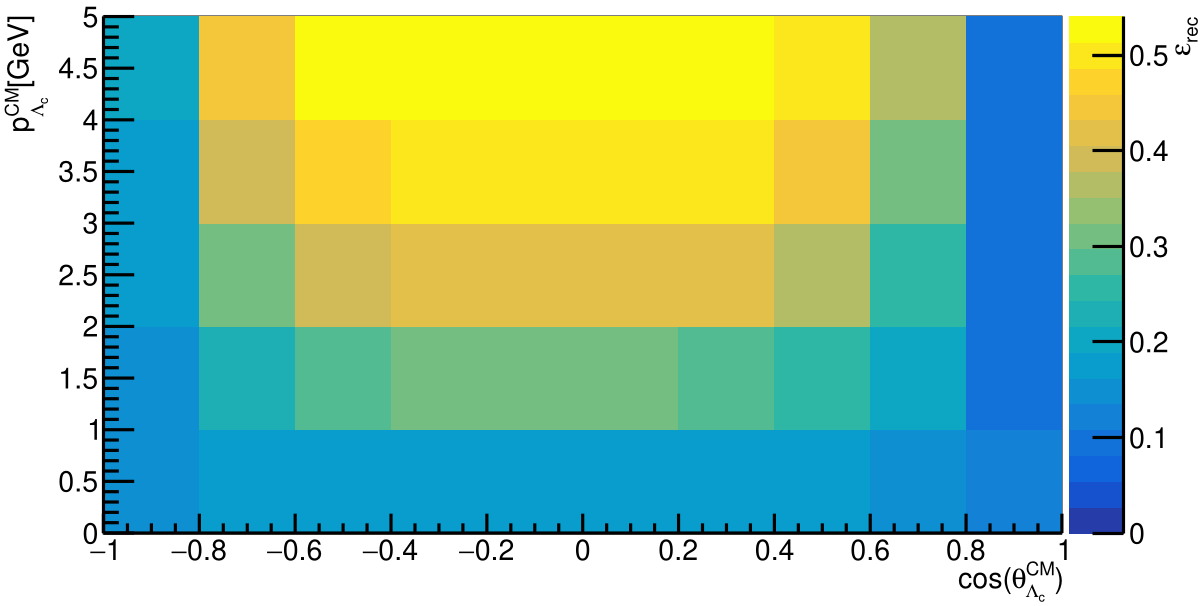
\includegraphics[width=1\linewidth]{img/l_l_nu_rec.png}
    \caption{Эффективность реконструкции распадов $\Lambda_c \to \Lambda e \nu_e$ в зависимости от
    косинуса полярного угла и величины импульса $\Lambda_c$-бариона в системе центра масс.}
    \label{l_l_nu:rec}
\end{figure}


Результы подгонки параметров методом максимального прадоподобия изображены на рис. \ref{l_l_nu:fit}


\begin{figure}[H]
    \centering
    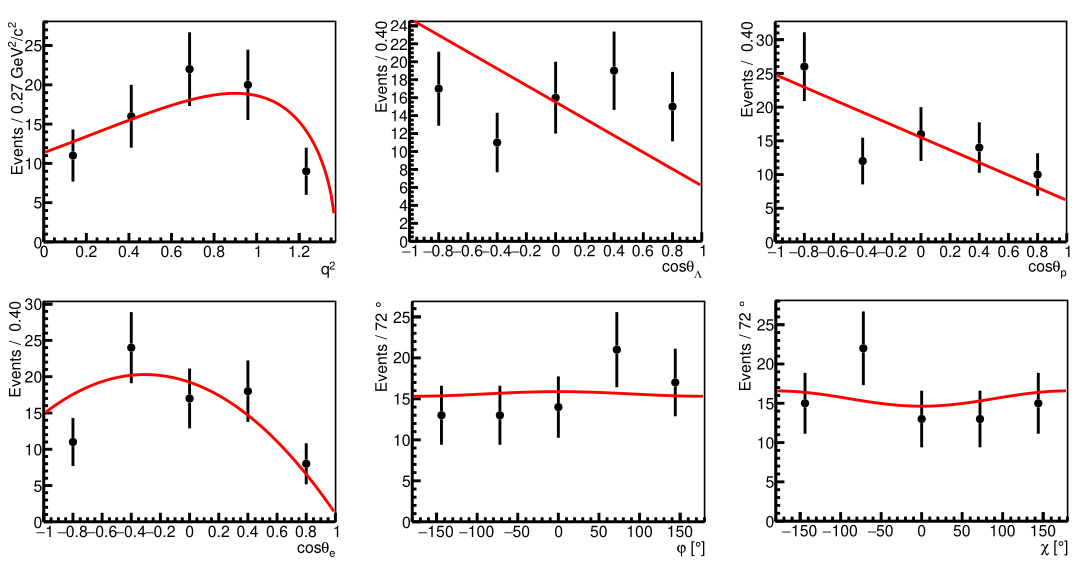
\includegraphics[width=1\linewidth]{img/l_l_nu_fit.png}
    \caption{Одномерные распределения событий $\Lambda_c \to \Lambda e \nu_e$ с наложенной
    функцией $f_{sig}$ с полученными параметрами}
    \label{l_l_nu:fit}
\end{figure}

\begin{eqnarray}
    \lambda_c \to \Lambda e \nu_e: \ R = -0.52 \pm 0.13,\ M_{pole} = 1.82 ± 0.19 GeV
\end{eqnarray}



